\section{Method}

This section describes our approach to solving the pagerank estimation problem. We present our methodology as we have applied it to the problem at hand, as opposed to extracting the generic, underlying principles, as these are mostly covered in the background section of this document.

The pagerank estimation problem is, given a webpage represented as an attributed graph with screenshots, to estimate the global popularity of that webpage.
Our ground-truth for \textit{popularity} is a list containing 100,000 webpages, created by Open PageRank.
More details can be found in Section \ref{OpenPageRank}.
The given data has several characteristics which have influenced our way of tackling the problem:

\begin{itemize}
    \item With approximately 100,000 samples, there is plenty of data available. The number of images is even higher, since a single sample can consist of up to 16 images.
    \item The problem is a ranking task. Samples need to be ordered and during inference the rank of a (possibly) unseen sample must be predicted. Besides the webpage ranking list (containing rank and domain) there is no information available.
    \item Images make up the majority of the information contained in the dataset. Neural networks, in particular convolutional neural networks (CNNs; see \cite{lecun1989backpropagation}) are performing well at processing images and at extracting features from them. With \cite{krizhevsky:imagenet} they have become the de-facto standard way of solving image classification problems where ever large datasets are available.
    \item The samples are variably-sized and can be easily represented as a graph: The number of screenshots taken from a domain may vary depending on the number of subpages. Links between subpages can be represented as edges in a graph. Naturally, the samples can be seen as graphs and a model capable of using the entire information from the graph seems best suited.
    \item The data is relatively noisy, e.g. samples might be mostly black or ranks might be inaccurate (as they are subject to change over time anyways).
\end{itemize}

Motivated by the stated observations, we decided to use a combination of CNN and graph network (GN) (see \cite{deepmind:graphnets}), trained with ranking loss functions, to predict pageranks.

Learning features as opposed to hand-engineering them seems reasonable as it is unknown to us what the visual elements are that distinguish popular and unpopular webpages. Furthermore, a dataset containing more than 1,000,000 images provides more than enough training data to work with high-capacity models, capable of learning complex features.

While many of today's CNN-papers deal with natural images, e.g. \cite{gu2018ava,szegedy2017inception,openai:learningdexterity}, there have been applications with computer generated images as well. \cite{beltramelli:pix2code} converts a screenshot into a fixed size feature vector. Therefore, CNNs seem very suitable for screenshot processing as well and are our choice.

Graph networks are suitable for dealing with the image graph. Arbitrary size, arbitrary pieces of information (we use only images, theoretically text, etc. can be used as well).

Ranking problem requires special losses.

We define an accuracy metric that allows us to evaluate the performance of our model. It measures how accurate the model ranks any two given webpages from a subset of the dataset relative to each other.

While our dataset contains webpages from domains which are (or have been) publicly available on the web, we want it to work with unseen inputs as well. The goal of our model's inference mode is to either estimate the absolute popularity of a webpage with respect to the top 100,000 webpages or, secondly, compare two (or more) given webpages relative to one and another.

\begin{figure}
    \centering

    \begin{tikzpicture}[]

        \draw[dashed] (0,-1) rectangle (6,1);
        
        % inputs and outputs
        \node (in_data) at (-1,0.5) [draw,process]{Dataset};
        \node (in_inference) at (-1,-.5) [draw,process]{Inference};
        \node (out_loss) at (7,1) [draw,process]{Loss};
        \node (out_accuracy) at (7,0) [draw,process]{Accuracy};
        \node (out_rank) at (7,-1) [draw,process]{Rank};
        
        % processing
        \node (cnn) at (1,0) [text width=1.65cm, align=center, draw, process]{Screenshot feature extractor};
        \node (gn) at (3,0) [text width=1.5cm, align=center, draw, process]{Graph network};
        \node (pred) at (5,0) [draw, process]{Output};

        % edges
        \draw[->] (in_data) -- (cnn);
        \draw[->] (in_inference) -- (cnn);
        \draw[->] (cnn) -- (gn);
        \draw[->] (gn) -- (pred);
        \draw[->] (pred) -- (out_loss);
        \draw[->] (pred) -- (out_rank);
        \draw[->] (pred) -- (out_accuracy);

    \end{tikzpicture}
    \caption[Webpage rank prediction model architecture overview]{Overview of the components of our webpage rank prediction model. Input to the model is either the pagerank dataset or one/several samples during inference. The model processes the inputs with the screenshot feature extractor, here a convolutional neural network (CNN), followed by a graph network which deals with the graph structure of the data, yielding a fixed-size output. The output is used to compute loss and accuracy (when training), or estimate a rank (during inference). The dashed box separates the model from the components orchestrating it.}
    \label{fig:methodcomponents}
\end{figure}

The remainder of this section describes the components of our model in greater detail. Figure \ref{fig:methodcomponents} gives an overview.

\subsection{Screenshot Feature Extractor}

The screenshot feature extractor is a component in this model. Its task is to extract a vector of fixed size from a given website screenshot. The vector is supposed to contain a condensed version of the information contained in the original image. Condensed with respect to the specific task the feature extractor is trained on.

The idea of feature extraction is a reoccurring scheme in the field of deep learning. Recurrent neural networks such as LSTMs (\cite{hochreiter1997lstm}) can extract a fixed size vector from a variable length sequence, used e.g. to map a sentence into a representation space, see e.g. \cite{salesforceabstractivesummarization}. Similarly, CNNs are used to extract features from images: It is a common architectural choice to classify an image with a CNN, the feature extraction, followed by fully connected layers, referred to as classification head, see e.g. \cite{krizhevsky:imagenet,szegedy2017inception,Girshick15:fastrcnn}. We borrow this idea and extract feature vectors from screenshots, which are the input to our model. The extracted features serve as input to the following stage, a graph network.

Mathematically, a screenshot feature extractor is a function mapping a screenshot into a smaller vector space: $f:\mathbb{R}^{480\times270\times3}\rightarrow\mathbb{R}^{32}$. We are working with two different types of screenshots, namely desktop and mobile webpage screenshots. The screenshots are similar in that they contain similar content (a website), however, potentially of different size. Also, mobile screenshots might have a different look overall, commonly having a menu drawer in the corner and a single-column layout. We decide to process a tuple of corresponding mobile and desktop screenshots with a single function to share some of the function's parameters. Specifically, the employed feature extractor is a function \begin{equation}
f_\text{dm}:\left(\mathbb{R}^{480\times270\times3},\mathbb{R}^{187\times333\times3}\right)\rightarrow\left(\mathbb{R}^{32},\mathbb{R}^{32}\right)\,,
\end{equation} where \enquote{dm} stands for desktop-mobile. The input tensors are two screenshots (desktop and mobile respectively), with three color channels. The output is a tuple consisting of two vectors. They are supposed to be mappings of the screenshot into a 32-dimensional feature space.

\begin{figure}
    \centering
    \begin{tikzpicture}[>=stealth, thick]
    \node (I_d) at (2,-16) [draw, process, align=flush center]
        {Desktop screenshot\\$\tens{I}_\text{d}\in\mathbb{R}^{480\times270\times3}$};
    
    \node (I_m) at (6,-16) [draw, process, align=flush center]
        {Mobile screenshot\\$\tens{I}_\text{m}\in\mathbb{R}^{187\times333\times3}$};
    
    \node (block1_d) at (2,-14) [draw, double, align=flush center]
    {Block1\_d\\$n_\text{filters}=32$};

    \node (block1_m) at (6,-14) [draw, double, align=flush center]
    {Block1\_m\\$n_\text{filters}=32$};

    \node (block2_d) at (2,-12) [draw, double, align=flush center]
    {Block2\\$n_\text{filters}=64$};
    \node (block2_m) at (6,-12) [draw, double, align=flush center]
    {Block2\\$n_\text{filters}=64$};

    \node (block3_d) at (2,-10) [draw, double, align=flush center]
    {Block3\\$n_\text{filters}=128$};
    \node (block3_m) at (6,-10) [draw, double, align=flush center]
    {Block3\\$n_\text{filters}=128$};

    \node (block4_d) at (2,-8) [draw, double, align=flush center]
    {Block4\\$n_\text{filters}=256$};
    \node (block4_m) at (6,-8) [draw, double, align=flush center]
    {Block4\\$n_\text{filters}=256$};

    \node (dense_d) at (2,-6) [draw, double, align=flush center]
    {Dense\\$n_\text{units}=256$};
    \node (dense_m) at (6,-6) [draw, double, align=flush center]
    {Dense\\$n_\text{units}=256$};

    \node (dense2_d) at (2,-4) [draw, double, align=flush center]
    {Dense\_d\\$n_\text{units}=32$};
    \node (dense2_m) at (6,-4) [draw, double, align=flush center]
    {Dense\_m\\$n_\text{units}=32$};

    \node (feat_d) at (2,-2) [draw, process, align=flush center]
        {Desktop feature vector\\$\bm{x}_\text{d}\in\mathbb{R}^{32}$};
    
    \node (feat_m) at (6,-2) [draw, process, align=flush center]
        {Mobile feature vector\\$\bm{x}_\text{m}\in\mathbb{R}^{32}$};
    
    \draw[->] (I_d) -- (block1_d);
    \draw[->] (I_m) -- (block1_m);

    \draw[->] (block1_d) -- (block2_d);
    \draw[->] (block1_m) -- (block2_m);
    \draw[dashed,<->] (block2_m) -- (block2_d);

    \draw[->] (block2_d) -- (block3_d);
    \draw[->] (block2_m) -- (block3_m);
    \draw[dashed,<->] (block3_m) -- (block3_d);

    \draw[->] (block3_d) -- (block4_d);
    \draw[->] (block3_m) -- (block4_m);
    \draw[dashed,<->] (block4_m) -- (block4_d);

    \draw[->] (block4_d) -- (dense_d);
    \draw[->] (block4_m) -- (dense_m);
    \draw[dashed,<->] (dense_m) -- (dense_d);

    \draw[->] (dense_d) -- (dense2_d);
    \draw[->] (dense_m) -- (dense2_m);

    \draw[->] (dense2_d) -- (feat_d);
    \draw[->] (dense2_m) -- (feat_m);
    
    \end{tikzpicture}
    \caption[Illustration of the feature extractor]{Illustration of the feature extractor; inputs are at the bottom, outputs at the top. Blocks with double borders are parameterized, dashed arrows indicate parameter sharing. The weight sharing between inner layers allows for similar, yet different feature extraction because the weight matrices of the first convolutional block and the last dense block are not shared.}
    \label{fig:featextr}
\end{figure}

We model the function $f_\text{dm}$ with a CNN. The high-level architecture is described and visualized in Figure \ref{fig:featextr}. Each \textbf{Block} consists of the following components:
\begin{enumerate}
    \item 2D convolutional layer with $n_\text{filters}$ filters, preserving the spatial size of the tensor and increasing the number of channels.
    \item ReLU activation function, $\operatorname{relu}(x)=\max(0,x)$.
    \item Second 2D convolutional layer with $n_\text{filters}$ filters, preserving all dimensions size of the tensor.
    \item ReLu activation function.
    \item 2D max-pooling with a kernel size of $(3,3)$. This reduces the spatial size of the tensor by a factor of $3$ along both width and height.
    \item 2D dropout (\cite{srivastava2014:dropout}) with drop probability $p_\text{drop}$, enabled during training, disabled during evaluation and inference.
\end{enumerate}
Exceptions to this are the first block which has a max-pooling size of $(2,2)$ and the fourth block which is followed by global average pooling. The \textbf{Dense} blocks each contain a fully connected layer followed by ReLu activation and dropout, except the last layer outputs the raw result of the matrix multiplication.

The parameters of the feature extraction model can be trained with backpropagation. The following modes of training are conceivable:
\begin{itemize}
    \item \textbf{End-to-end training}. The feature extractor ist trained alongside with the other components of the model, gradients are computed by backpropagating through the following components. This method will train the CNN such that the extracted vectors contain features most helpful/relevant for the overall task. The downside is the additional computational complexity introduced by backpropagating through a graph network.
    \item \textbf{Pre-training without fine-tuning}. The weights of the feature extractor are learned on a separate auxiliary task and transferred to be used for the actual problem. This method requires an auxiliary task, which (in this setting) may be the prediction of a pagerank based solely on a single desktop-mobile screenshot tuple. If the model parameters are kept frozen, i.e. are not being fine-tuned, once the entire model is trained on the main task, the feature vectors for the dataset can be cached so the computational overhead of passing images through the CNN can be omitted, thereby greatly increasing the training speed. Even though the described auxiliary task is similar to the pagerank prediction based on an entire graph of screenshots, its difference may lead to slightly less meaningful feature vectors.
    \item \textbf{Pre-training with fine-tuning}. Same as \textit{Pre-training without fine-tuning} except the weights are kept trainable and are fine-tuned on the main task as well. Caching of feature vectors is not possible.
\end{itemize}

\subsection{Graph Network Blocks}

Where the GN blocks are positioned in the model, first layer to make use of the graph structure, nodes are from feature extractor. Inputs and outputs, formal definition.

Baseline GN block; maps to scalar and aggregates. Intuition: looking a single images and ranking based on them + avg. +figure

Full GN block; more complex: Block definition with concat and avg/max aggregation. Dense layers everywhere. Reflexive graph for avg (to avoid 0 edge count). +figure

Intuition behind the block: Information flows, global state is sort of an aggregation.

Weight-sharing between consecutive blocks or not.

Conversion into a fixed-size output using the global attribute (output block).

Interpretation of the feature extractor as a special kind of block, bring up the encoder-core-decoder scheme from the GN DeepMind example.

(potentially +figure, if it adds any value)

\subsection{Loss Function}

Loss function is in a ranking setting. We chose pairwise because initial experiments showed that pointwise resulted in unstable training. Derive the loss function in the following.

Dataset vector, computation of the output matrix, ..., weighting w

Sum aggregation, final loss scalar normalized

Additional weighting term w, chosen as bla bla, with log base. Plot with linear and log in comparison (axis: 1-100k, 0-1). Intuition is that the top 10k samples contain more information than the e.g. 80k-90k.

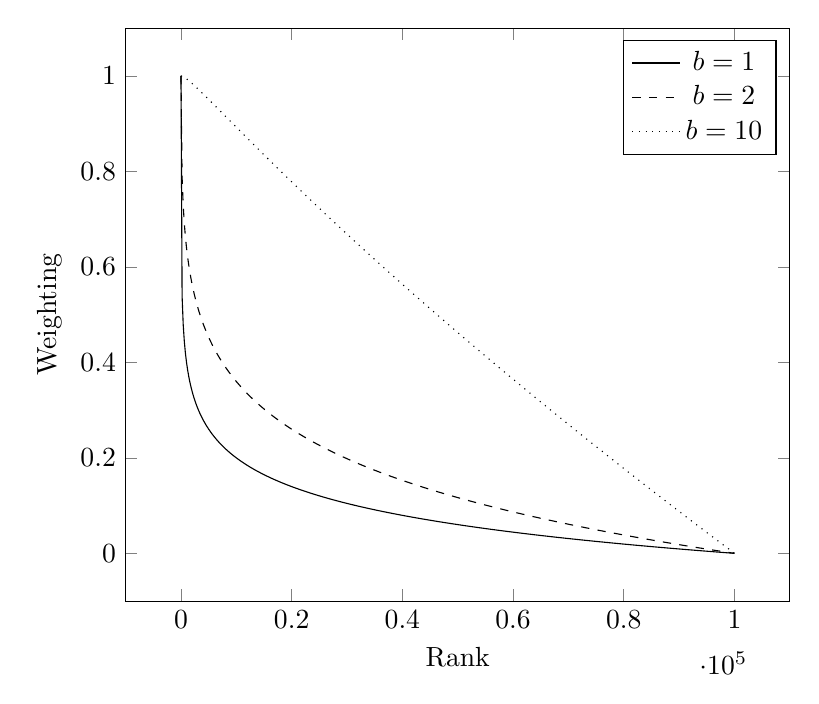
\begin{tikzpicture}

    \pgfplotsset{
        scale only axis,
    }

    \begin{axis}[
        xlabel=Rank,
        ylabel=Weighting,
        samples=500,
        ]
        \addplot[][domain=1:100000]{1-pow(ln(x*100000) / ln(100000) - 1., 1)};
        \addlegendentry{$b=1$}
        \addplot[style=dashed][domain=1:100000]{1-pow(ln(x*100000) / ln(100000) - 1., 2)};
        \addlegendentry{$b=2$}
        \addplot[style=dotted][domain=1:100000]{1-pow(ln(x*100000) / ln(100000) - 1., 10)};
        \addlegendentry{$b=10$}
    \end{axis}

\end{tikzpicture}

Approximation with mini-batches, number of comparisons grows quadratically so larger batches are desirable. Also regularizing effect, as always.

Note that this is single scalar supervision (or binary classification) and it effectively trains a CNN.

\subsection{Evaluation Metrics and Inference}

Accuracy is computed by feeding all samples through the model, large vec. Then matrix and ground-truth matrix comparison. Number of correct pairwise results.

Advantage: Can be easily compared to humans, however difficulty is not taken into consideration, e.g. 80,001 and 80,000 are extremely hard/impossible. Band of growing width that masks out the close samples.

Formal definition of inference, i.e. sample $x$ to rank or pairwise and listwise. 

Pairwise: feed both samples, magnitude of difference is certainty, sign is relative ranking.

Pointwise: requires ground truth, pairwise with everyone, come up with something here...
